%TODO

\section{Introduction}

Wazuh is different than base OSSEC in that it adds capabilities (a RESTFul API and rules and decoders) and is easier to install (it uses the ELK stack to gather and preprocess data, while OSSEC leaves that choice to the user).
\begin{figure}[H]
  \centering
	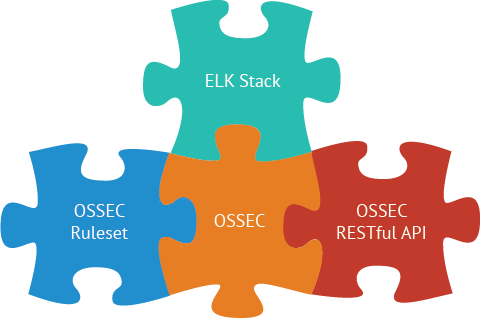
\includegraphics[width=.6\textwidth]{figuras/wazuh_stack.png}
	\caption{The different parts of Wazuh\cite{wazuh_stack}}
\end{figure}
\linej
The most interesting qualities of Wazuh for this project are\cite{wazuh_index}\cite{wazuh_documentation}: %necessary redundancy
\begin{itemize}
	\item \textbf{Rootkits detection}: Rootkits are commonly used after an attack has suceeded to use the computer of the victim leaving no traces.
	\item \textbf{File integrity monitoring}: It can provide detection of intrusions by identifying changes in content, permissions, ownership, and attributes on the monitored files. It can be used to comply with GDPR (General Data Protection Regulation).
	\item \textbf{Scalability and multi-platform}: This means that the work on this project could really be used in real work environments.
	\item \textbf{Configuration management}: The configuration is managed by the Wazuh server (Wazuh manager) and the agents can be grouped, allowing custom, grupal or global gathering and detection for each agent.
	\item \textbf{Multiple sources of data}: The scanned data can be from logs, output of commands or databases. %TODO more?
	\item \textbf{Active response}: An automated remediation to security violations and threats, to mitigate more the possible damage. For example to stop the Internet connection to isolate a compromised system.
	\item \textbf{Improved ruleset}: This reduces the workload of this project, as it can serve as guidance and complement some of the rules and decoders that this project intends to create or modify.
	\item \textbf{Open source, free and easy to contribute to}: This is optional but nice, as it offers a chance to an unexperienced student to contribute in a real and useful project. The project is hosted on Github and Google Groups. In this project the contribution would be to the ruleset\cite{wazuh_ruleset} and not to the core of Wazuh\cite{wazuh} or the documentation\cite{wazuh_documentation2}.
\end{itemize}
\linej
The RESTFul API interacts using OSSEC commands and would be interesting if this project were related to a tool issuing queries to Wazuh, but this is not the case. Anyway it is still something valuable to have as these kind of tools are very common nowadays.

\linej
\linej
Wazuh provides support and integration with multiple important tools and technologies:
\begin{itemize}
	\item Docker container for OSSEC: An ossec-server image with the ability to separate the ossec configuration/data from the container.
	\item Puppet and Ansible: For massive deployment. This can be very helpful to setup a big environment mostly because even being no need to put configuration files in the agents for Wazuh often is necessary to configure other things and the process of registering agents can be tedious manually.
	\item Network IDS integration: Gives the option to use OwlH and integrate Suricata and Bro to generate alerts in Wazuh.
	%\item Splunk infrastructure: Comprised of a Splunk Enterprise instance as indexer and a Splunk Forwarder node, as well as the Wazuh app for Splunk.
	\item VirusTotal: A free virus, malware and URL online scanning service that combines more than 40 antivirus solutions.
	\item OSQuery: Osquery can be used to expose an operating system as a high-performance relational database. This allows you to write SQL-based queries to explore operating system data.
\end{itemize}
\linej
The use of these depends on the scenario and the only one we take interest in is VirusTotal, because it can work as a secondary detection method for the most critical or complicated cases.

\section{Wazuh architecture}

A basic Wazuh setup has the next components\cite{wazuh_architecture}:
\begin{itemize}
	\item Wazuh server: Runs the Wazuh manager, API and Filebeat (Filebeat is only necessary in distributed architecture). It collects and analyzes data from deployed agents.
	\item ELK stack: It reads, parses, indexes, and stores alert data generated by the Wazuh server. The ELK stack is flexible, highly configurable and very used in big data.
	\item Wazuh agent: Runs on the monitored host, collecting system log and configuration data and detecting intrusions and anomalies. It talks with the Wazuh server to which it forwards collected data for further analysis.
\end{itemize}
\linej
The main difference with the architecture of OSSEC is the ELK stack, because OSSEC leaves the choice of tools to the user. ELK stands for the combination of:
\begin{itemize}
	\item Elasticsearch: Gets the data and allows search queries and analysis.
	\item Logstash: Transforms the data to the desired format. This step can make alike data from different log and output formats, trivializing the decoders work.
	\item Kibana: Shows the data in a web browser, with graphs and options like grouping and time interval. This is often easier than to write commands to scan the OSSEC log in the Wazuh server, as the data of interest tends to stay the same.
\end{itemize}
\linej
There are two possible architectures for this setup: having the ELK stack in the same machine that the Wazuh server (singlehost) or in a separated one (distributed). Each has advantages and disadvantages and in this project we will use the singlehost because in our case there are no constraints and is easier to set up and is more efficient.
\begin{figure}[H]
  \centering
	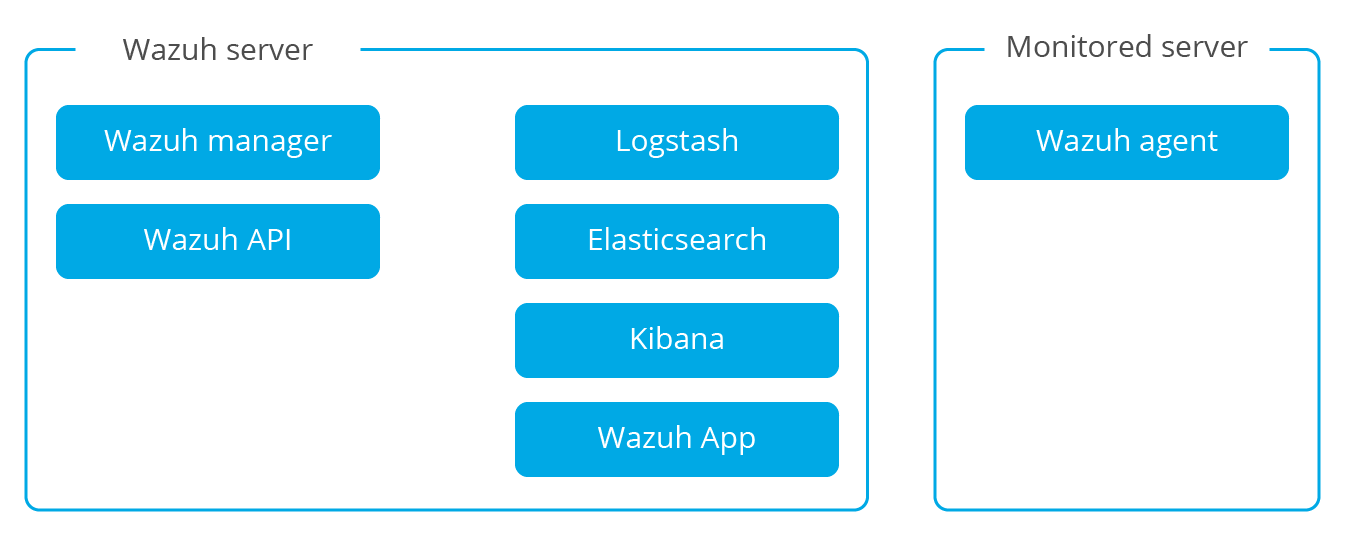
\includegraphics[width=\textwidth]{figuras/wazuh_singlehost.png}
	\caption{Singlehost architecture}
\end{figure}

\begin{figure}[H]
  \centering
	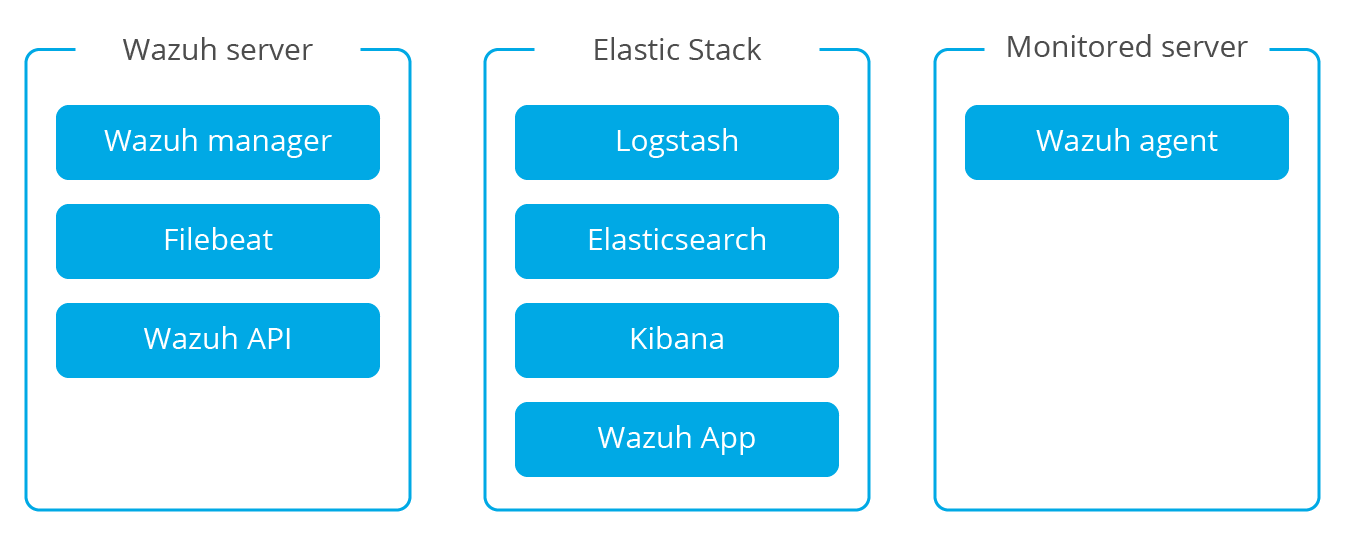
\includegraphics[width=\textwidth]{figuras/wazuh_distributed.png}
	\caption{Distributed architecture}
\end{figure}
\linej
To understand better the communications and data flow in Wazuh we will now get into more detail on the process\cite{wazuh_architecture2}\cite{wazuh_data_flow}.
\linej
\linej
Wazuh agents use the OSSEC message protocol to send collected events to the Wazuh server over port 1514 (UDP or TCP). The Wazuh server then decodes and rule-checks the received events with the analysis engine. Events that trip a rule are augmented with alert data such as rule id and rule name. The Wazuh message protocol uses a 192-bit Blowfish encryption with a full 16-round implementation, or AES encryption with 128 bits per block and 256-bit keys.
\linej
Logstash formats the incoming data and optionally enriches it with GeoIP information before sending it to Elasticsearch (port 9200/TCP). Once the data is indexed into Elasticsearch, Kibana (port 5601/TCP) is used to mine and visualize the information.
\linej
The Wazuh App runs inside Kibana constantly querying the RESTful API (port 55000/TCP on the Wazuh manager) in order to display configuration and status related information of the server and agents, as well to restart agents when desired. This communication is encrypted with TLS and authenticated with username and password.

\begin{figure}[H]
  \centering
	\makebox[\textwidth][c]{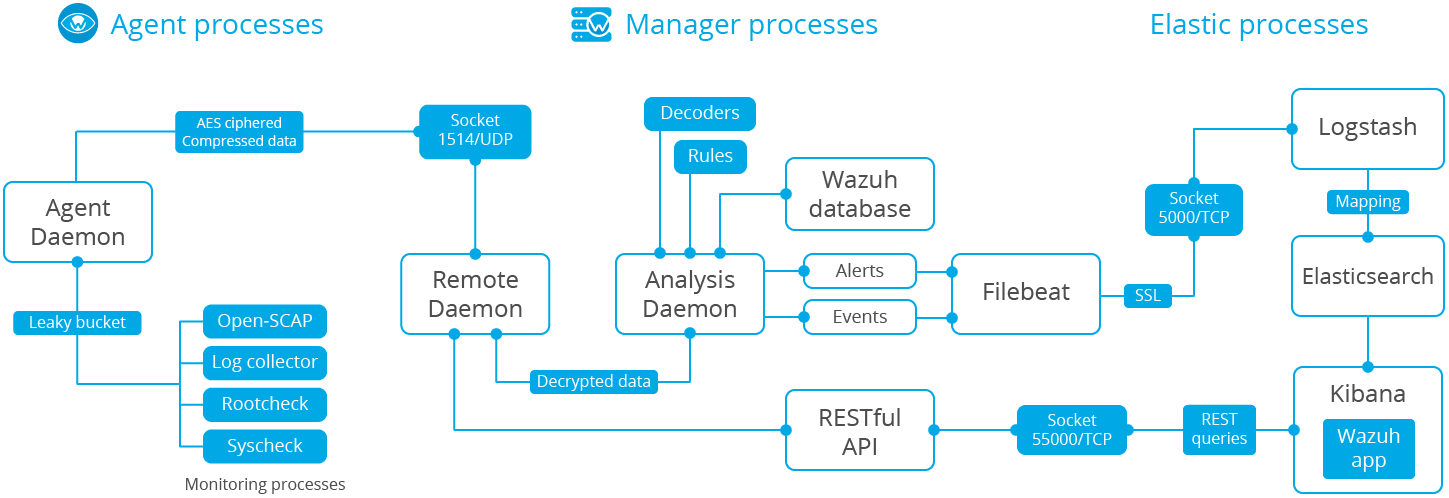
\includegraphics[width=1.2\textwidth]{figuras/wazuh_data_flow1.png}}
	\caption{Communications and data flow}
\end{figure}
\linej
Both alerts and non-alert events are stored in files on the Wazuh server in addition to being sent to Elasticsearch. These files can be written in JSON format and/or in plain text format (.log, with no decoded fields but more compact). These files are daily compressed and signed using MD5 and SHA1 checksums.


\section{Rules and decoders}
They constitute the main part of this project and they can be used to detect application or system errors, misconfigurations, attempted and/or successful malicious activities, policy violations and a variety of other security and operational issues\cite{wazuh_index}. Wazuh is quite helpful with the features and documentation of the ruleset and in this project the already existing rules and decoders were a great help as examples.
\linej
\linej
Rules can be added in \textit{/var/ossec/etc/rules/} and decoders in \textit{/var/ossec/etc/decoders/} without any issue, but to change the already existing ones in \textit{/var/ossec/ruleset/rules/} or \textit{/var/ossec/ruleset/decoders/} is a bad idea because the next changes in those files from updates would overwrite them. The solution is to copy the code (actually only the id is needed) of the existing item to the folder where we can add new ones, make the desired changes add \textit{overwrite=``yes''}\cite{wazuh_custom}.
\linej
\linej
As mentioned before Wazuh adds its own ruleset over the one provided by the OSSEC project. The next table shows about 20\% of the combined ruleset that Wazuh uses, where ``Out of the box'' means that the source was the OSSEC project.
\begin{figure}[H]
  \centering
	\makebox[\textwidth][c]{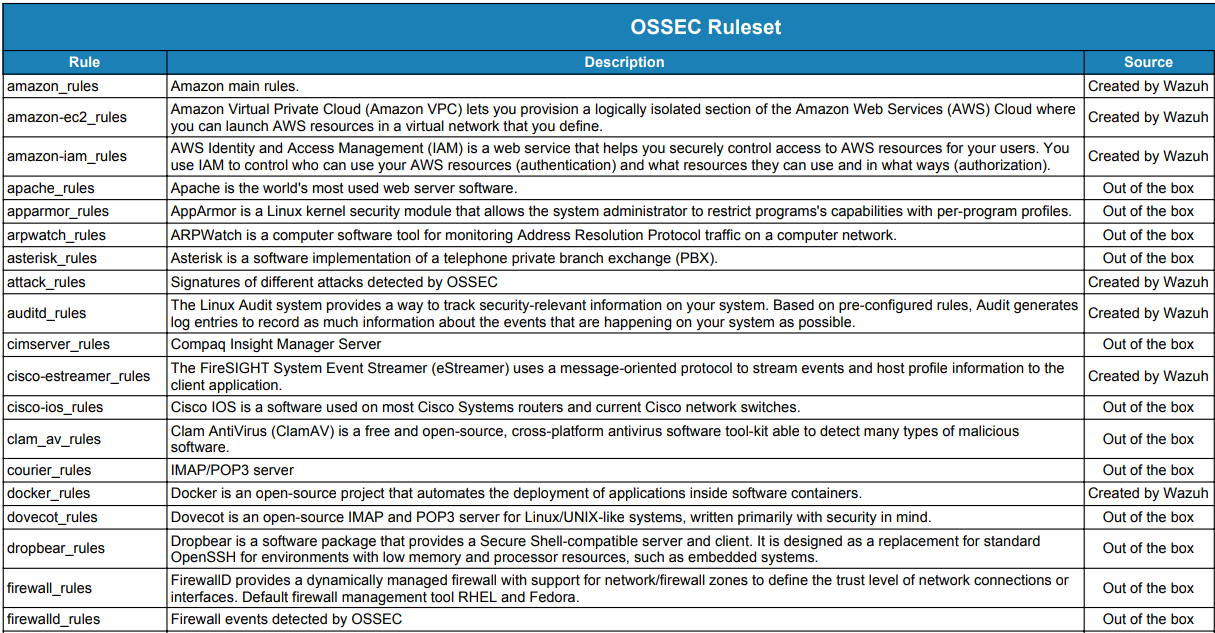
\includegraphics[width=1.1\textwidth]{figuras/wazuh_ruleset.png}}
	\caption{Portion of the ruleset used by Wazuh\cite{wazuh_ossec_ruleset}}
\end{figure}
\linej
Wazuh provides a way to manually test how an event is decoded and if an alert is generated with the tool \textit{/var/ossec/bin/ossec-logtest}\cite{wazuh_testing}, which is very useful for debugging. To use it you only need to introduce the data as it would be in the wild (in the logfile or command output). This command provides the option ``-v'' that shows which rules are tried and which trigger an alert. This tools does not no need a restart of the wazuh-manager service whenever changes want to be tested because it reads the configuration directly. But is also worth to mention that some times it can be missleading because it does not work the exact same way as the manager, for example the logtest may show that the log matches a certain rule but actually it has matched a previous one silently.
\linej
\linej
For example for this input:
\linej

\includegraphics[width=\textwidth]{figuras/ossec-logtest_input.png}
\linej
We get the next output:
\begin{figure}[H]
  \centering
	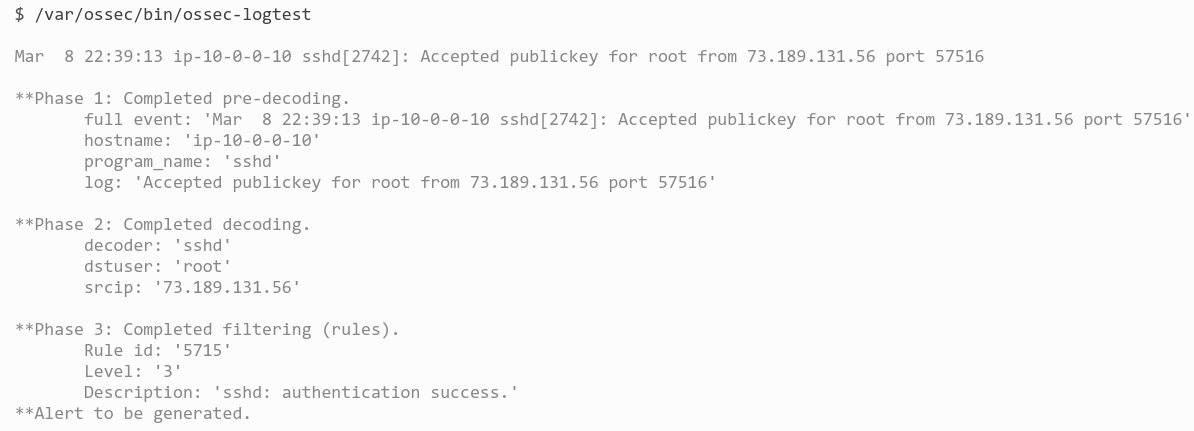
\includegraphics[width=\textwidth]{figuras/ossec-logtest_output.png}
	\caption{Example of output for ossec-logtest}
\end{figure}
\linej
%TODO cambiar currently in version
After version 3.0.0 (we are currently in 3.9) Wazuh incorporates an integrated decoder for JSON logs enabling the extraction of data from any source in this format. This can be very useful in many situations, for example trivializing the generation of alerts for Suricata (without the need for a decoder just for Suricata)\cite{wazuh_json}.
\linej
\linej
Another interesting feature is to check if a field extracted during the decoding phase is in a CDB list (constant database). The main use case of this feature is to create a white/black list of users, IPs or domain names.\cite{wazuh_cdb}.
